\chapter{Results and analysis}
%Plan St 1
%In this chapter we showcase a series of results from the {\sc meqsilhouette} simulator. We begin with canonical simulations from the ISM, atmospheric and pointing error modules. Following this, we present the result of a typical calibration and imaging procedure in the presence of a variable source and a variable troposphere.
In this chapter we will showcase a series of results from the {\sc meqsilhouette} simulator in order to demonstrate it's capabilities and predictions.


\section{Canonical simulations}\label{sec:can_sim}
{\it Author's note: This section draws largely from the work of \citet{Blecher_2016}.}

\subsubsection{ISM variability and substructure}
%st 1
We remind the reader of the reproduction of the ISM-induced closure phase uncertainty result \citep{Ortiz_2016}, shown in Fig.~\ref{fig:substructure2}. To obtain this result we simulated 50 observations, each with an independent realisation of the ISM scattering screen. The success of the reproduction verifies a large section of the simulation software, including I/O, the interferometric and the ISM modules. 

%st1
Following the discussion on the ISM theory (section~\ref{sec:ism_scat}), we compare predictions of the ensemble-averaging regime, which consists of only a Gaussian convolution, and the average regime, which includes the presence of stochastic substructure. Note that the ensemble-average is invariant with time and would not bias the closure phase of a point-symmetric source.
%st1
\begin{quotation}  
``We present the results of a simulated observation of 10 minutes duration at 14:00 UTC on four consecutive days in Fig.~\ref{ISM_sequence}. To compare to published observations, we use the three-station EHT array consisting of the Submillimeter Telescope (SMT) in Arizona, the Combined Array for Research in Millimeter-wave Astronomy (CARMA) in California and the James Clerk Maxwell Telescope (JCMT) on Mauna Kea, Hawaii. The relative transverse velocity between the observer and scattering screen is set to $50~\rm{km\,s}^{-1}$ to be consistent with \citet{Ortiz_2016}. The source is a circular Gaussian with a $\rm{FHWM}=40$~$\mu$-arcsec, approximately the angular distance that a scattering screen would travel over $\sim 4$~days. The source size has been chosen such that it is consistent with the latest estimate of the size of Sgr~A$^\star$ at $230$~GHz \citep{Fish_2011}.  Closure quantities are model dependent and calculated as specified in \citet{Rogers_1995}, where the thermal noise was added based on the system equivalent flux density (SEFD) table in \citep{Lu_2014}.


Fig.~\ref{ISM_sequence} provides an example of closure phase and flux variability over a 4 day period using a static source. Accurate simulation of the ISM-induced closure phase variation is essential in order to make any inference on asymmetric, event-horizon scale structure \citep[e.g.][]{Fish_2016,Ortiz_2016}. This will become even more important as the EHT sensitivity increases by an order of magnitude in the near future when [phased ALMA is included in the array.]''
\citep{Blecher_2016} 
\end{quotation}

%to do : expand the analysis of the simulation out ?? not sure how
%st 1
This simulation clearly shows how the longest baselines are more sensitive to the refractive substructure, which in turn strengthens the challenge of imaging compact features and/or fine structure like the BH shadow. 


%%orbiting hot spot st1
Recalling the variability associated with Sgr~A* (section~\ref{sec:variability}), if the source has intrinsic spatial variability, e.g. an orbiting hotspot model \citep{Doeleman_2009} or jet shocks, this will increase ISM variability as the relative motion between source, screen and observer is increased \citep{Blecher_2016}. Although an orbiting plasma blob might be torn apart on sub-orbit timescales by differential rotation and the non-linear shear of the Magneto-Rotational Instability \citep[(MRI)][]{Balbus_1991}, this scenario becomes more of a physical possibility when resonant orbits are considered \citep{Brink_2015}. A resonant orbit occurs when the ratio of characteristic radial $\omega_r$ and longitudinal frequencies $\omega_\theta$ is a rational number $\omega_r/\omega_\theta = n/m$, where $n,m \in \mathbb{N}$. A hotspot in such an orbit could be stable against differential rotation and associated shearing. In the case of Sgr A*, the $1/2$ and $2/3$ resonances have  length scales of 41 and 55~$\mu$-arcsec respectively for a Schwarschild BH \citep{Brink_2015}, which is observable with the EHT. Also note that these resonant length scales are greater than $r_{\rm ref} \sim 10\ \mu$-arcsec and so the orbit would traverse independent refractive substructure fluctuations. This is relevant to methods like that demonstrated in \citet{Doeleman_2009} which rely on periodic closure phases. The periodic signal would exist (albeit altered by the ISM) but only on timescales less than $t_{\rm ref}$, assuming the orbiting body is unresolved.


%polarisation st 1 
Finally, we note that the ISM is polarisation invariant, hence the variability of polarisation ratios will not be biased by ISM scattering. Methods which use polarisation ratios \citep[e.g.][]{Johnson_2014} allows for valuable insight into how the source variability and ISM variability could be separated.



%st1
\begin{figure}[h!]
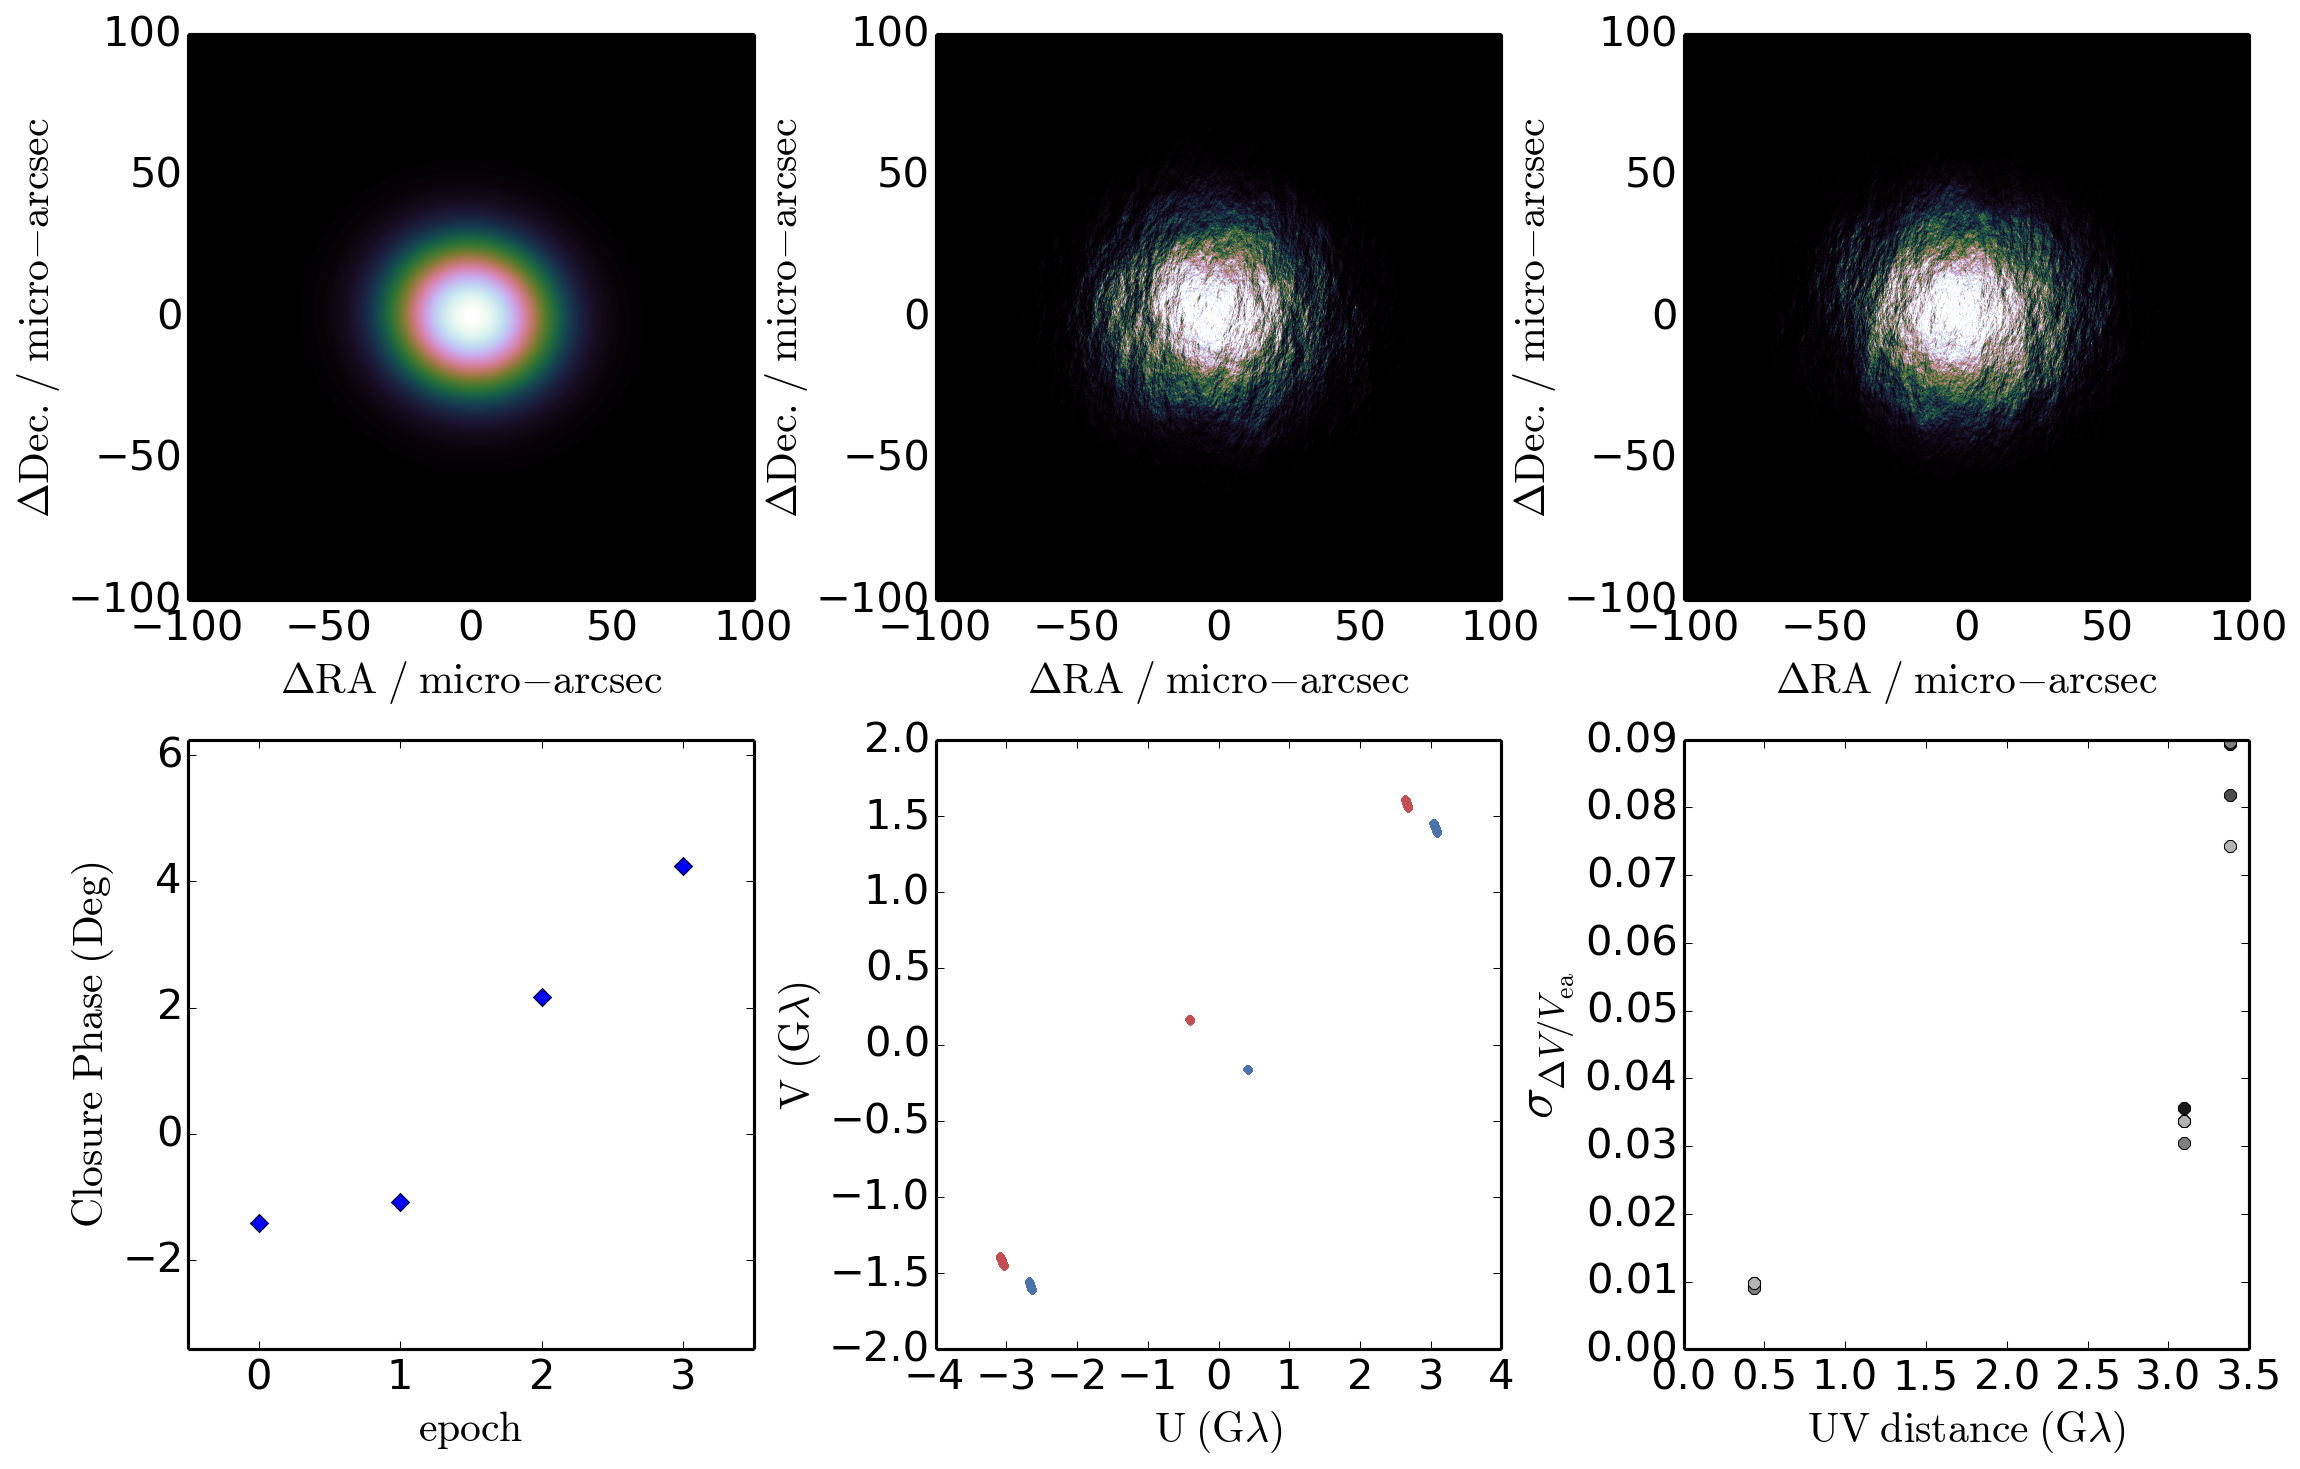
\includegraphics[width=\columnwidth]{Images/ism}
\caption{``An example simulation of ISM scattering towards Sgr~A$^{\star}$, observed with SMT-JCMT-CARMA.  The top panel, left to right, shows the original $\rm FWHM = 40$~$\mu$-arcsec Gaussian {\bf (top left)}, the simulated ISM scattered image on the first night {\bf (top middle)} and last night {\bf (top right)} of the observation, respectively.  The bottom panel, left to right,  shows the evolution of the 10 minute-averaged closure phase with epoch {\bf (bottom left)}, {\sl uv}-tracks for each night {\bf (bottom middle)} and the RMS fractional visibility amplitude differences $\sigma_{\Delta V /V_{\rm ea}}$ as a function of {\sl uv-}distance {\bf (bottom right)}. $ \Delta V= (|V_{\rm a}|-|V_{\rm ea}|)$, where $|V_{\rm a}|$ and $|V_{\rm ea}|$ are the simulated average and ensemble average visibility amplitudes respectively. Variations from the ensemble-average flux on the shortest baselines reveal total flux modulation while flux variations on longer baselines and non-zero closure phases track the fluctuations in substructure.''(Image and caption reproduced from \citet{Blecher_2016}) \label{ISM_sequence}%
}
\end{figure}

\subsubsection{Atmospheric transmission and scattering}

%st1
As described in section~\ref{sec:trop_imp}, the implementation of the tropospheric module is separated into mean and turbulent components. For the mean atmosphere, we simulate opacity, sky brightness temperature and time delay as a function of site weather, elevation angle and frequency. The most important climate parameters are precipitable water vapour column depth (PWV), ground temperature and ground pressure. The turbulent module simulates Guassian fluctuations in the time delay $\tilde{t}$ arriving at each station, where $\sigma(\tilde{t})$ is based on Kolmogorov turbulence on a two-dimensional scattering screen.


%Opacity + Brightness temperature st 1 - leave for now
The first atmospheric result we present are mean opacities and sky brightness temperatures for ALMA, the Submillimeter Array (SMA) and the South Pole Telescope (SPT) at 230~GHz, shown in Fig.~\ref{fig:mean_atm}. These sites were chosen as they are all considered excellent sites for sub-mm astronomy and form an essential part of the EHT. The PWV ranges used were taken from the 25th and 75th percentile data shown in \citet{Lane_1998} and is in good agreement with the measured opacities therein. %The ground% where I got the pressure/temp data from? I think it was SPT -lane 1998, ALMA - website/aatm defaults, SMA - site memo

%st 1
\begin{figure}[h!]
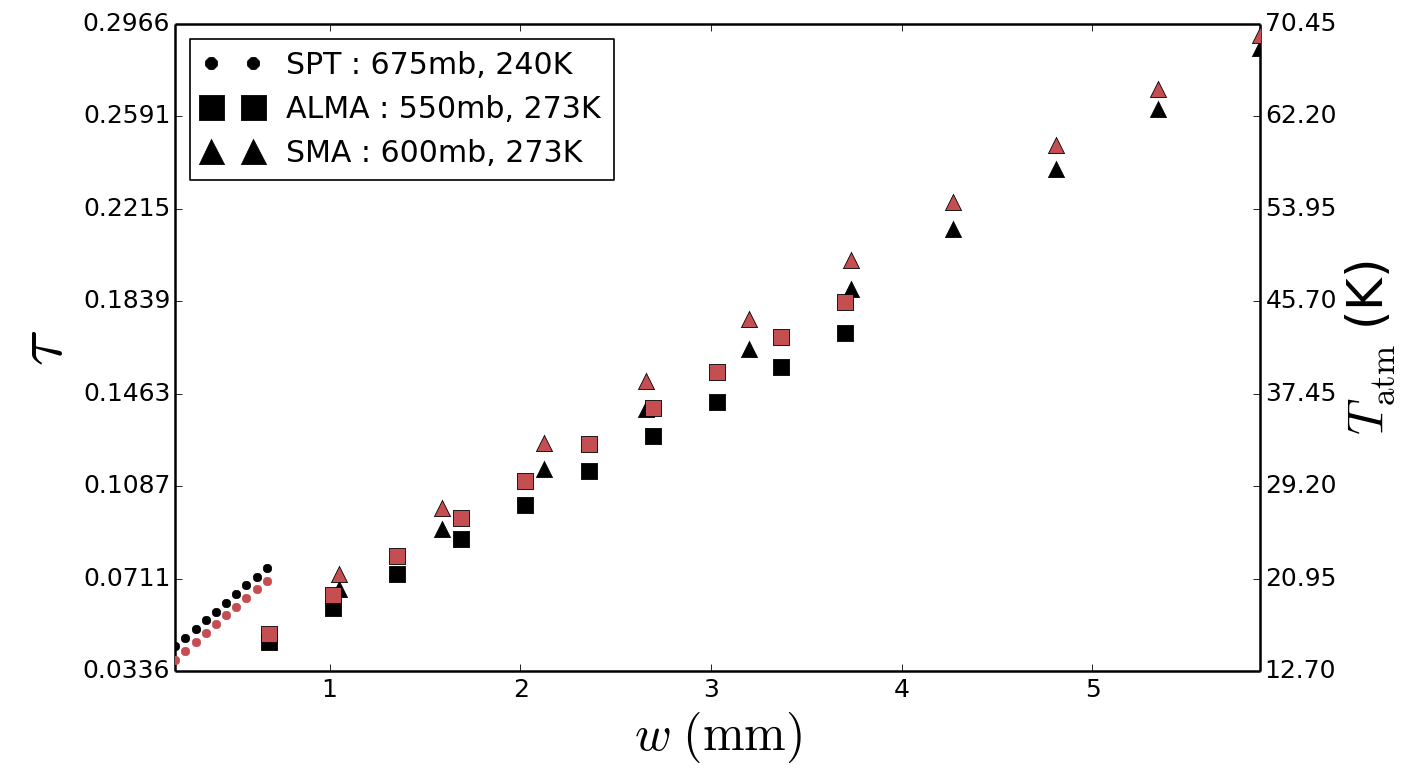
\includegraphics[width=1.\columnwidth]{Images/opacity}
\caption{``Simulated mean opacity (black) and sky brightness temperature (red) at $\nu =230$~GHz  for three typical ground pressures and temperatures over a typical PWV range \citep{Lane_1998} which approximately represent the sites of SPT (dots), ALMA (squares) and SMA (triangles). The legend shows the estimated input ground (pressure, temperature) parameters for each site.''(Image and caption reproduced from \citet{Blecher_2016})\label{fig:mean_atm}%
}
\end{figure}

%st 1 -a bit silly that I didnt do any 'bad' sites like PDBI or something like that
Immediately apparent is that the opacity and sky brightness temperature both exhibit linear relationships with respect to PWV content. Furthermore, opacity and sky brightness temperature are proportional to ground pressure and inversely proportional to the ground temperature \citep{Pardo_2001}. It is also clear that SPT has far less opacity, and a lower sky brightness temperature than ALMA and the SMA which are fairly similar. A comparison of the thermal receiver temperatures for the three sites  (ALMA$\sim262$~K,  SMA$\sim327$~K, SPT$\sim 255$~K) reveals that for the thermal noise contribution from the receiver is approximately an order of magnitude higher than sky brightness temperature. 



%Turbulent and mean delay st 1
Of vital importance to an interferometric site is atmospheric stability. An example of the effects of atmospheric transmission and scattering on the time delay $\tilde{t}$ at 230~GHz is shown as a function of observation time in Fig.~\ref{delay_plots}. Canonical values (see caption) were used for the weather parameters. It is apparent that the turbulent component is typically 3-4 orders of magnitude lower than the mean delay, even though the coherence time is on the order of seconds.


%st1
\begin{figure}[h!]
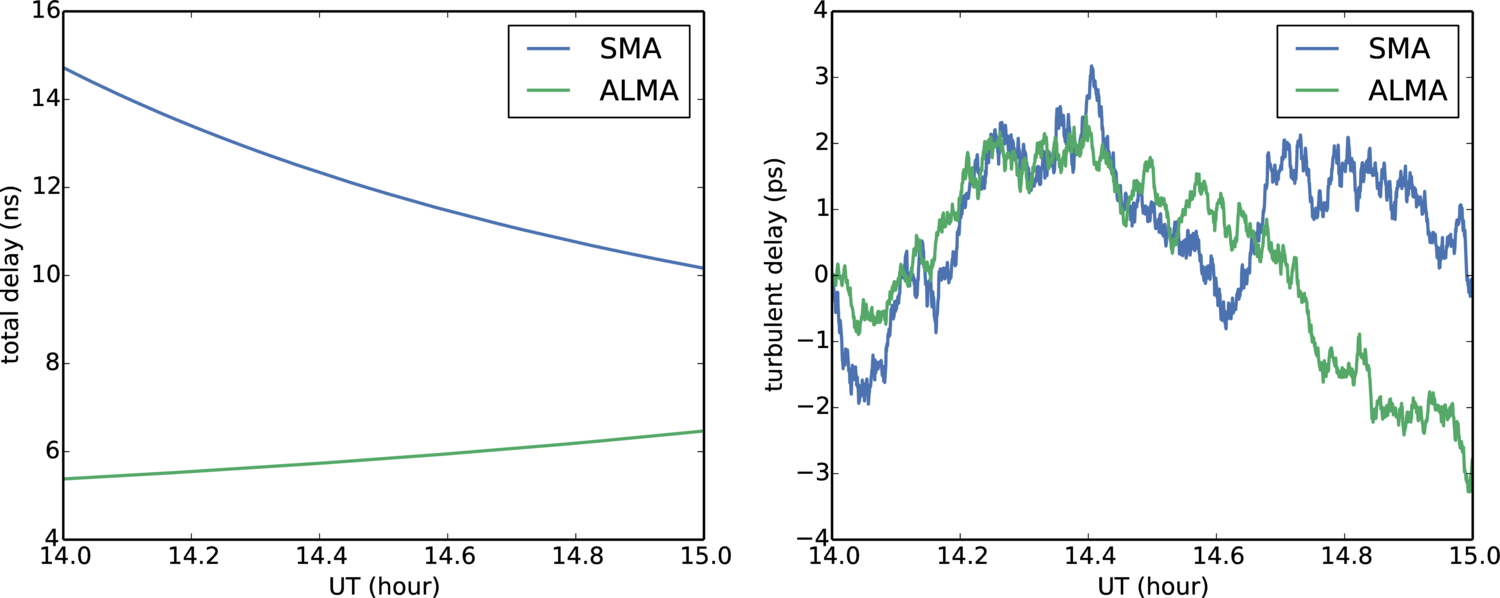
\includegraphics[width=\columnwidth]{Images/delays}
\caption{``Simulation of the total delay (left) and the turbulent atmospheric delay (right) for SMA (blue) and ALMA (green) sites towards Sgr~A$^\star$. Ground pressures and temperatures are the same as Fig.~\ref{fig:mean_atm}, precipitable water vapour above each station is set to $w=2$~mm, and the instantaneous zenith coherence time is set $T_0=10$~s for both stations. Note that all tropospheric parameters are, however, independently set. The conversion from time delay to phase at 230~GHz is $1$~rad~$=0.7$~ps.''(Image and caption reproduced from \citet{Blecher_2016})\label{delay_plots}%
}
\end{figure}



%Trop images
\begin{quotation}
``We now investigate the effect of the tropospheric module on image quality for various levels of calibration accuracy. We simulate the simple scenario of a sky model that consists of a 2.4~Jy point source at the phase centre, which is an approximate EHT-measured flux density of Sgr~A$^\star$ at 230~GHz. We assume a zenith phase coherence time of $t_0=10$~s above each station (however, each stations PWV can be independently simulated). We approximate the effect of imperfect calibration by adding a small fraction of the turbulent phase noise. For this example, we do not include the mean delay component, assuming it to be perfectly corrected for during the calibration. Imaging [is performed] using the two dimensional inverse fast Fourier transform''\\
\citep{Blecher_2016}
\end{quotation}

%Trop images
\begin{figure}[h!]
\includegraphics[width=\columnwidth]{Images/trop_images}
\caption{``The effect of residual troposphere phase noise on interferometric images of a point source observed for 12 hours at 230~GHz with 4~GHz bandwidth with the following array : SPT, ALMA, SMA, SMT, LMT and JCMT, assuming the same SEFDs as \protect\citet{Lu_2014} and an elevation limit of 15$^\circ$. For simplicity the weather parameters at each station were set to: coherence time $t_{\rm 0}=10$~sec; PWV depth $w=1$~mm; ground pressure $P=600$~mb; ground temperature $T =273$~K. {\bf Top left:} interferometric map with thermal noise only. {\bf Top right:} atmospheric attenuation and sky noise (due to non-zero opacity) with 1\% of the turbulent phase noise added. {\bf Bottom left:} as previous but with 3\% of turbulent phase contribution. {\bf Bottom right:} as previous but with 6\% turbulent phase contribution. The fractional turbulent phase contributions are illustrative of the effect of fringe-fitting errors. The black crosshairs indicate the original source position. ''(Image and caption reproduced from \citet{Blecher_2016}) \label{fig:trop_images}%
}
\end{figure}


%st 1 - attenuation of flux
Analysis of the images reveal increasing attenuation in the original peak, central flux due to the simulated residual calibration errors. In the calibration procedure, station gains cannot be solved for on arbitrarily short intervals as adequate SNR is needed to fringe-fit/self-calibrated. Aside from the fact that solutions are imperfect, within a given solution interval, there will also be a degree of uncalibrated turbulence-induced phase fluctuations.

Specifically, the flux of original central peak component is reduced to $76.5\%$ (attenuation only - not shown in plot), $75.1\%$ (1\% turbulence), 65.5\% (3\% turbulence) and  40.5\% (6\% turbulence). In the case of 6\% turbulence, the imaging artifact vertically below the source at 44.5\% of the original source flux becomes brighter than the corrupted source. 


%offset in original source st 1
Furthermore, there are slight offsets in the central peak flux from the original source position as shown by progressive movement away from the black crosshairs. This shift $\approx 5.6\ \mu$-arcsec at 6\% turbulence. 


%st 1
The residual calibration errors also distort the interferometric artifacts (as seen in the uncorrupted image), which result from inadequate sampling of the Fourier domain before imaging. This distortion causes a breakdown in image-plane deconvolution and source finding algorithms as the Point Spread Function (PSF) is difficult to subtract and the interferometric artefacts are difficult to distinguish from source structure. This further weakens the ability of such source finding algorithms to extract, with high fidelity, the BH shadow feature.


%Absence of blurring st 1
There was no evidence of blurring or a loss of resolution in the simulated images of Fig.~\ref{fig:trop_images}. Blurring can result if the decoherence is considered proportional to baseline length, as longer baselines would be less coherent and so their visibility amplitudes are effectively downweighted. For the EHT, as different stations experience completely independent phase fluctuations, the baseline length of the VLBI baselines will not be correlated with the magnitude of the decoherence. Alternatively, the blurring consequence, characteristic in optical single dish telescopes as 'seeing', is induced by the overlaying of many speckled images of the source \citep{Narayan_1992} across the scattering disc. This does not seem to occur in the interferometric image reconstruction with the inverse fourier transform. The reason being that the phase noise of each fourier mode is Gaussian, and so positional deviations of each Fourier mode from zero phase noise effectively cancel in the image domain. Hence attentuation but no blurring.


%Incoherent closure phases.. This section is needed to link up to the discussion on closure phase uncertainty in the mm-VLBI section. Yep worth mentioning. but leave this 

%NON-CLOSING ERRORS
%Non-closing errors due to incoherent averaging - "no conjugates for triples" - possibly comes down to how one defines SNR. In the definition used in the literature we followed, they assumed only gaussian noise, which was not the case..A better definition would be to look at the distribution of a number of samples 
%maybe just a mention of how the closure phase uncertainty could change.

\subsubsection{Antenna pointing offset}

%mild intro


\begin{quotation}
``We investigate the effect of pointing errors on the 50~m (i.e. fully illuminated) Large Millimeter Array (LMT) dish configured in an eight station VLBI array. The LMT has been measured to have an absolute pointing accuracy of $\sigma_{\rm abs} = 1-3$~arcsec, where smaller offsets occur when observing sources closer to zenith, and a tracking pointing accuracy $\sigma_{\rm track} < 1$~arcsec\footnote{http://www.lmtgtm.org/telescope/telescope-description/}. We investigate the observational effect of these errors through three different pointing error models which explore different instructive and plausible scenarios. The LMT has been singled out due to its narrow primary beam and that it may serve as a reference station for the EHT array given its sensitivity and central geographic location. 

The source used is a circular Gaussian of characteristic size $\Theta_{\rm src}=50$ $\mu$-arcsec, located at the phase centre. For this investigation, as long as $\Theta_{\rm src} \ll \theta_{\rm PB}$, the exact structure of the source is unimportant. We approximate the LMT beam profile using an analytic WSRT beam model (equation~\ref{eq:wsrt_beam}) with a factor of two increase in the beam factor $C$ to take into account the increased dish size of the LMT. [Hence] $C_{\rm LMT} \approx 130$~GHz$^{-1}$. Note that the power beam $EE^H$ becomes $\cos^6$, resulting in a $\rm{FWHM} = 6.5 $~arcsec at 230 GHz.


We make use of the RMS fractional visibility amplitude error $\sigma_{\Delta V/V_0}$, where $V_{\rm PE}$ and $V_{0}$ are the visibility amplitudes with and without pointing errors respectively, and  $\Delta V = V_{\rm PE} - V_{0}$.
\\
\citep{Blecher_2016}
\end{quotation}

%the different pointing models
For this simulation we use three different pointing error models, as introduced in section~\ref{sec:instrument}. Firstly, we simulate a simple \emph{constant} pointing offset. For the second case, we simulate a smooth, \emph{sinusoidal} pointing error to replicate a tracking error. The period of the sinusoid is sampled from a uniform distribution between 0.5 and 6 hours, and a peak amplitude $A_{\rho} = \sqrt{2} \sigma_{\rho}$ , where the factor $\sqrt{2}$ relates the peak amplitude to the RMS of a sinusoidal, zero-mean waveform.  In the third case, we simulate \emph{stochastic} variability which replicates slewing from source/calibrator to source/calibrator, where the pointing error is re-sampled every 10 minutes from a Gaussian of characteristic width equal to the quoted pointing error. This simulation is repeated for 50 realisations for each pointing offset to generate reasonable uncertainties \citep{Blecher_2016}. In Fig.~\ref{fig:pointing}, $\sigma_{\Delta V/V_0}$ is plotted against pointing error $\rho$ over the range $0 \le \rho \le 4.5$~arcsec for the three classes of error. Note that although plotted on the same set of axes, $\rho$ represents slightly different quantities for each of the three simulations.

%analysis : why LMT, and phased array
\begin{quotation}
``We only consider LMT pointing errors due to its narrow primary beam and potential to be used as a reference station. However, the capability to simulate independent pointing errors for each station is available. In the case of a phased array, a pointing error simulation could be used to investigate the contribution of the pointing error to a variable phasing efficiency, which can be reasonably approximated by a scalar Jones matrix.''\\
\citep{Blecher_2016}
\end{quotation}


\begin{figure}[h!]
\includegraphics[width=\columnwidth]{Images/point_Crop}
\caption{``RMS relative amplitude error induced by pointing error with the 50~m (i.e. fully illuminated) LMT antenna as a function of pointing error offset $\rho$ at 230~GHz. We assume that these errors are degenerate or non-separable from the self-calibration/fringe-fitting model used. See text for the description of the three models used. This simulation capability enables constraints on the magnitude of pointing-induced errors given a particular pointing calibration strategy.''(Image and caption reproduced from \citet{Blecher_2016})\label{fig:pointing}%
}
\end{figure}
\

\begin{quotation}
``Visibility amplitude errors due to antenna pointing error has been investigated for the $50$~m  LMT dish operating at $230$~GHz. In Fig.~\ref{fig:pointing}, we show that pointing errors associated with frequent phase centre switching (stochastic variability) could introduce a RMS fractional amplitude error $\sigma_{\Delta V/V_0} \sim 0.1 - 0.4$ for an absolute pointing accuracy  $\sigma_{\rm abs} \sim 1-3$~arcsec. In contrast, tracking errors are less problematic with $\sigma_{\Delta V/V_0} \le 0.05$ for a tracking accuracy  $\sigma_{\rm track}<1$~arcsec. The case of a constant error pointing model is comparable to that of the `slow variability' case. If the gain error is non-separable from the calibration model used, it could be interpreted as intrinsic variability, substructure and/or increased noise. If unaccounted for, this effect has the potential to limit the dynamic range of mm-VLBI images. Further tests to constrain the pointing uncertainties of EHT stations will lead to more accurate interferometric simulations and hence the overall impact on black hole shadow parameter estimation. Here we demonstrate the capability to incorporate a range of plausible pointing error effects into a full simulation pipeline. For future observations at 345~GHz, these effects will be even more pronounced, given the narrower primary beam.\\
\citep{Blecher_2016}
\end{quotation}





%\subsubsection{Performance?}
%Performance/speed



%\section{Fringe-fitting test}
%leave until done
%First we fringe fit and image a stationary point source and compare to the result in Fig.~\ref{fig:trop_images}. 
% In an upcoming paper, we perform a systematic exploration of the turbulent tropospheric effects on the accuracy of fringe-fitting algorithms/strategies, through use of an automated calibration procedure and including the added complexity of a time-variable source.


\section{Future work and other applications}\label{sec:improv}

\subsubsection{Anomalous pointing error}
There is another class of pointing error which we did not include in our simulation, but which should be folded in through a combination of the tropospheric and antenna pointing modules. This effect is called the `anomalous refraction' and is due to the time-variable phase-gradient across the aperture \citep[e.g.][]{Holdaway_1997,Butler_1997,Holdaway_1998}. This is essentially the first order fluctuation in water vapour across the dish diameter $d_{\rm dish}$ (i.e. a wedge) and hence will be a function of $D_{\phi}(d_{\rm dish})$. These are pointing errors which will change on the timescale $d_{\rm dish}/v \sim 1-50$~s for $10<d_{\rm dish}<50$~m and $1<v<10$~m/s, where $d_{\rm dish}$ is the diameter of the aperture.  

\citet{Holdaway_1998} derive the standard deviation of the pointing error as a fraction of beam width,
\begin{equation}
 \sigma_{\rm pe}(d_{\rm dish}),\theta) = \frac{\sqrt{2 D_l(d_{\rm dish})}}{\sqrt{\sin\theta}\lambda},
\end{equation}
where $l$ is the extra electric path length and $\theta$ is the elevation angle. Hence in terms of fractional beam size, the effect goes as $d_{\rm dish}^{\beta/2}$ and hence the effect for large dishes will be larger amplitude variations (as shown by Fig.~\ref{fig:pointing}) over longer time periods. 


%Estimates of $\sigma_{\rm pe}$ shown in \citet{Holdaway_1998} range between $0.48-3.68$-arcsec, where the lower bound was calculated for an 8m dish, observing at zenith with relatively stable atmosphere and the upper bound was calculated for a 15m dish observing at $10^\circ$ with a relatively unstable atmosphere.  

Apertures which are fitted with water vapour radiometers are able to track the PWV distribution across the primary beam \citep{Lamb_1998}. However, most of the EHT stations are currently not fitted with radiometers and hence this effect could be tricky to calibrate.

\subsubsection{Testing calibration, imaging and parameter estimation}

%Testing and development of calibration, imaging and parameter estimation pipelines st 1
The primary use of synthetic data is to provide 'known' datasets on which to run calibration, imaging and parameter estimation pipelines. This can take the form of beauty contests, where various algorithms are utilised without knowledge of the true source and the results are compared post-facto. This is especially useful with imaging algorithms which have many `hand-tuned' parameters and difficulty with repeatability, uniqueness and fidelity of their solutions. Alternatively, one could perform a more systematic investigation of how an algorithm performs under a range different conditions. A key test which we have alluded to throughout this thesis is a systematic exploration of the turbulent tropospheric effects on the accuracy of fringe-fitting algorithms/strategies, including the added complexity of a time-variable source. A key point of such an investigation being the capability of assigning quantitative values to systematic and stochastic uncertainties across a wide range of physically relevant conditions.


%bayesian calibration
%An original motivation for the {\sc meqsilhouette} simulator was that it could eventually be implemented as a bayesian calibration routine where the signal corruptions were solved for. However, as many of the dominant signal corruptions have turned out to be stochastic and hence indeterminant, it no longer makes sense to go down this route. Indeed one would need a GPU-accelerated simulator to be able to sample the parameter space. Fortunately then, a collegue is planning a GPU bayesian calibration routine.  

%end-to-end st 2 - but you dont need an end- to end for some of this - but good enough 
With the current work developing automated fringe-fitters at JIVE (casa-based) and UCT/SKA-SA (bayesian) by Des Small and Iniyan Natarajan respectively, there arises the possibility of an end-to-end simulation pipeline, i.e. from theory to calibrated data product, within the next year. In this scenario, one could estimate the precision and accuracy with which the EHT could extract parameters (e.g. shadow size and asymmetry) in a range of canonical scenarios. This will also allow weak points in the calibration/analysis to be identified and subsequently improved as well as to determine which approaches to extracting science are more viable (e.g. analysis in the visibility domain vs image domain).
This argument can be extended to the realm of station upgrades (e.g. enhanced bandwidth) and the investigation into novel (sub)millimetre sites. 


%Data interpretation st1
As the EHT will be observing in a unique regime, there will always be doubt, double-checking and questioning of the interpretation of the data. This is especially the case with the use of closure quantities, where the recent result of an increase in closure phase with UT hour, measured on the Hawaii-Arizona-California triangle \citep{Fish_2016}, provides a good example. Simulations help formulate and test quatitatively plausible scenarios. For example the contribution of different components (e.g. ISM substructure, SNR) to the scatter in this result could be investigated for different source models. 

\begin{quotation}
``Significant progress has been made in the theoretical and numerical modeling of the inner accretion flow and jet launch regions near a supermassive black hole event horizon
\citep[e.g.][]{Zanna_2007,Etienne_2010,Dexter_2013,Moscibrodzka_2014, McKinney_2014}. As the sensitivity of the EHT stands to dramatically increase, these theoretical efforts must be complemented by advances in interferometric simulations. With \textsc{MeqSilhouette}, we now have the ability to couple these with sophisticated interferometric and signal propagation simulations.  Moreover, detailed interferometric simulations will enable us to quantify systematic effects on the black hole and/or accretion flow parameter estimation.''\\
\citep{Blecher_2016}
\end{quotation}



\subsubsection{A public online interface}
%st 1
Table~\ref{tab:parameters} shows the set of parameters needed to run a standard {\sc meqsilhouette} simulation. This moderate number of parameters ($24+6N_{\rm stations}$) can be quickly chosen or selected from a list, especially if most of the defaults are preset and unlikely to change. This speaks to the possibility of an online GUI interface which would provide the user with the capability to run standard simulations without having to delve into code. The capability to run such simulations would be useful to both theorists and observers in the broader AGN/SMBH/mm-VLBI community. For this reason, we trialed an online interface at the Leiden 2015 mm-VLBI workshop\footnote{http://www.astron.nl/other/workshop/mm-VLBI2015} with an early version of the {\sc meqsilhouette} simulator, which was well received by the researchers present. We are, however, yet to convert the latest version of the pipeline \citep{Blecher_2016} into such an interface, but hopefully this implementation will be made available in the future when matters relating to public/propriety status of the codebase are cleared up.


\subsubsection{Full Stokes}
%st 1
One of the key observables for the EHT is polarisation dependent quantities \citep{Johnson_2015b}. Although this version focused only on total intensity, if {\sc meqsilhouette} is taken up by members of the community, subsequent versions will enable the full Stokes cube as input. This should not entail much work as our chosen data formats (MS, {\sc fits}) as well as the FFT and UV sampling routine in {\sc MeqTrees} already support full Stokes logic including parallactic angle rotation. Signal propagation through the ISM and troposphere as well as antenna based complex gains errors are polarisation independent. The work would be primarly involve altering the existing scripts to deal with the book-keeping of the extra dimension. In addition the implementation of the associated signal corruption, polarisation leakage, is straightforward in the RIME formalism as it is simply an off-diagonal Jones matrix which is approximately constant over the course of an observation.

%\subsubsection{Opacity and atmospheric brightness temperature fluctuations}
% basically 
%In addition to tropospheric turbulence-induced phase errors, the turbulent contribution to variations in opacity is also important.
%Run multiple realisations of atm to link the phase fluctuations to opacity and brightness temperature fluctuations %possibly by fluctuating the input climate parameters., but this might be unfeasible.

























